\documentclass[letterpaper]{article}
    \usepackage{amsmath}
    \usepackage{tikz}
    \usepackage{epigraph}
    \usepackage{lipsum}
    \usepackage{float}
    \usepackage{glossaries}
    \usepackage{graphicx}
    \usepackage{imakeidx}
    \usepackage{hyperref}
    \graphicspath{{Images/}}
    \setcounter{tocdepth}{2}
    \makeglossaries
    \makeindex[columns=2, title=Alphabetical Index]
    \floatstyle{boxed}
    \restylefloat{figure}
    \renewcommand\epigraphflush{flushright}
    \renewcommand\epigraphsize{\normalsize}
    \setlength\epigraphwidth{0.7\textwidth}

    \definecolor{titlepagecolor}{cmyk}{1,.60,0,.40}

    \DeclareFixedFont{\titlefont}{T1}{ppl}{b}{it}{0.5in}

    \makeatletter
    \def\printauthor{%
        {\large \@author}}
    \makeatother
    \author{
        Sam Miller \\
       }

    % The following code is borrowed from:  https://tex.stackexchange.com/a/86310/10898

    \newcommand\titlepagedecoration{%
    \begin{tikzpicture}[remember picture,overlay,shorten >= -10pt]

    \coordinate (aux1) at ([yshift=-15pt]current page.north east);
    \coordinate (aux2) at ([yshift=-410pt]current page.north east);
    \coordinate (aux3) at ([xshift=-4.5cm]current page.north east);
    \coordinate (aux4) at ([yshift=-150pt]current page.north east);

    \begin{scope}[titlepagecolor!40,line width=12pt,rounded corners=12pt]
    \draw
      (aux1) -- coordinate (a)
      ++(225:5) --
      ++(-45:5.1) coordinate (b);
    \draw[shorten <= -10pt]
      (aux3) --
      (a) --
      (aux1);
    \draw[opacity=0.6,titlepagecolor,shorten <= -10pt]
      (b) --
      ++(225:2.2) --
      ++(-45:2.2);
    \end{scope}
    \draw[titlepagecolor,line width=8pt,rounded corners=8pt,shorten <= -10pt]
      (aux4) --
      ++(225:0.8) --
      ++(-45:0.8);
    \begin{scope}[titlepagecolor!70,line width=6pt,rounded corners=8pt]
    \draw[shorten <= -10pt]
      (aux2) --
      ++(225:3) coordinate[pos=0.45] (c) --
      ++(-45:3.1);
    \draw
      (aux2) --
      (c) --
      ++(135:2.5) --
      ++(45:2.5) --
      ++(-45:2.5) coordinate[pos=0.3] (d);
    \draw
      (d) -- +(45:1);
    \end{scope}
    \end{tikzpicture}%
    }




\begin{document}
\begin{titlepage}

	\noindent
	\titlefont Mumba\par
	\epigraph{A Project Mangement Solution\\ November 18, 2018}%
	{\textit{}\\ \textsc{}}
	\null\vfill
	\vspace*{1cm}
	\noindent
	\hfill
	\begin{minipage}{0.35\linewidth}
		\begin{flushright}
			\printauthor
		\end{flushright}
	\end{minipage}
	%
	\begin{minipage}{0.02\linewidth}
		\rule{1pt}{125pt}
	\end{minipage}
	\titlepagedecoration
\end{titlepage}
\tableofcontents
\pagebreak

\section{Introduction}

Mumba (https://mumba.azurewebsites.com) provides a simple no frills product management solution for small solo projects like those seen in university classes. My website is open to all and I hope that my project can be of use to myself and others in managing their projects and tasks. Anyone can register an account and use my application. Once the user has logged in they can boards which are collections of lists. They can then open the board and create tasks/cards in different lists to keep track of steps to complete a project. There currently is no user to user interactions, a board made by one user cannot be shared with any other user.

My Project is implemented as a full stack C\# ASP.Net Core application, I used the MVC pattern to dynamically manage the views returned to the users of my application. The buttons and interactions a user has with the website are controlled by one of the Four controller classes which will be detailed in the Description of Components section. The SQL server behind my web app is dynamically called to bring forth only the correct data that belongs only to the user who requested them. Each http request is routed to the proper controller's method for handling the request.

\section{Related Works}

The core functionality of Mumba is inspired by project boards (commonly known as  a kanban board) is commonly seen in Atlassian's Trello.com. Mumba is much simpler, there are not as many features as included in Trello, for example in Mumba's current state each board has 3 lists and only 3 lists, Trello dynamically allows creation and deletion of lists.

\section{System Architectural Design}

The system architecture follows the Model View Controller model of web design. The application was deployed across two Azure instances one is the platform as a service Web App Container that hosts my ASP.Net Core MVC web application, the second instance is a Windows Server Running an SQL Server. With a Azure web application a domain name is automatically registered, in my case my website can be reached at https://mumba.azurewebsites.net.

The views of my websize use Razor (HTML + C\# functionality) pages as a base and materialize css: https://materializecss.com as the basis for the look and feel of my website.

\subsection{Relational table: AppUsers}

\subsection{Relational table: Identity Users}

\subsection{Relational table: Boards}

\subsection{Relational table: Tasks}

\section{Detailed Description of Components}

The following is a detailed Description of each functional componet of the Mumba application, I have organized them by the Controller class that handles the requesst and response for each call. Each handled http request is directed to a controller and then a specific method of that controller. In most cases a new view is called but a small handful of cases do not return a view.
Invalid calls will result in a error page being displayed, and in order to view information beyond the register and login page one must be logged in.

\subsection{Account}
The Account controller handles session management and login/log out functionality.

\subsubsection{Login}
Takes a LoginRequest model that is generated by taking the username and password from the login views form and it will also grab a boolean value based off of the checkbox for session remembrance. It will then attempt to log the user in using the loginrequest model, if the request fails the user is redirected to the login page. If the login request succeeds then the user is sent to the BoardsController's All method. The following screenshot is of the Login page.


\begin{figure}[H]
  \centering
  \caption{The Login View}
  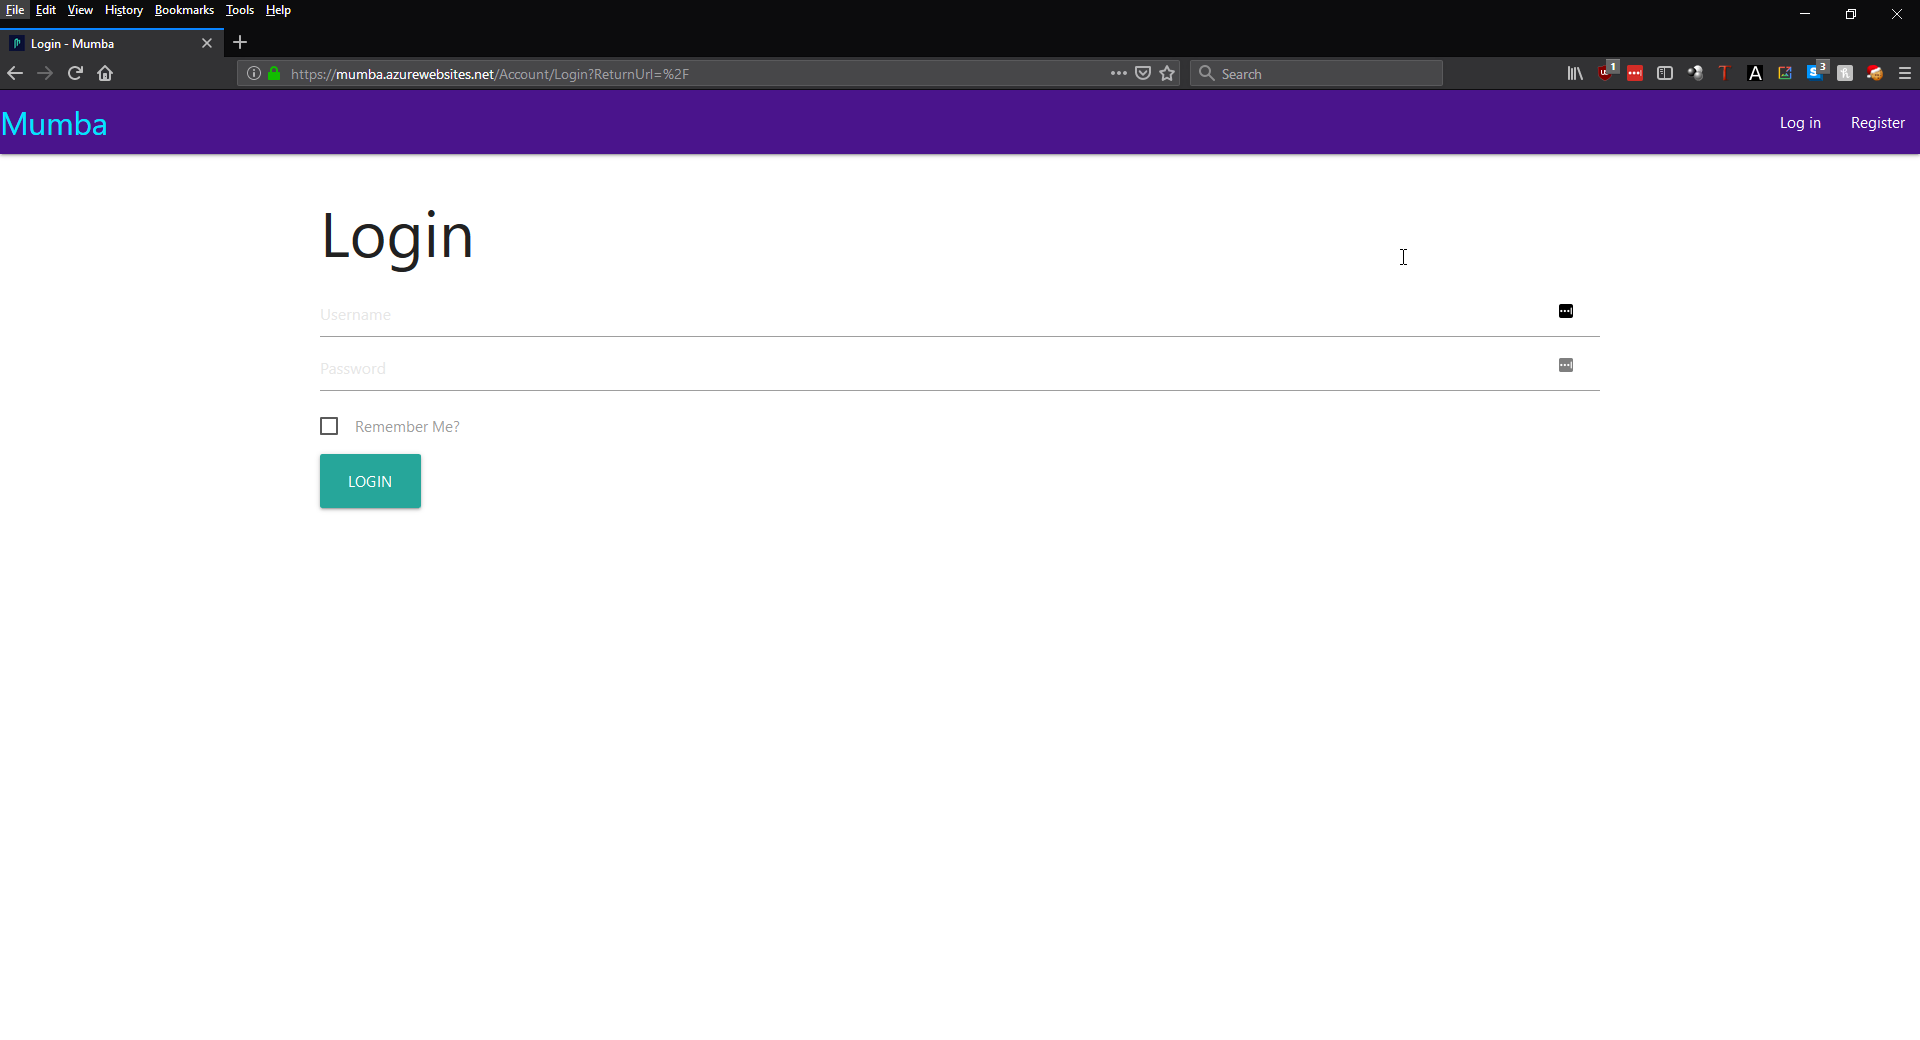
\includegraphics[scale=0.2]{Images/Login}
\end{figure}

\subsubsection{Logout}
This method ends a users session when called and redirects the browser to the login page.

\subsection{User}

The user controllers main function is to handle the creation of accounts. The information from the Registration pages form is loaded into a NewAppUser model and then passed to the userManager to have the account registered to the database. The following screenshot is of the User Registration page/view.

\begin{figure}[H]
  \centering
  \caption{The User Registration View}
  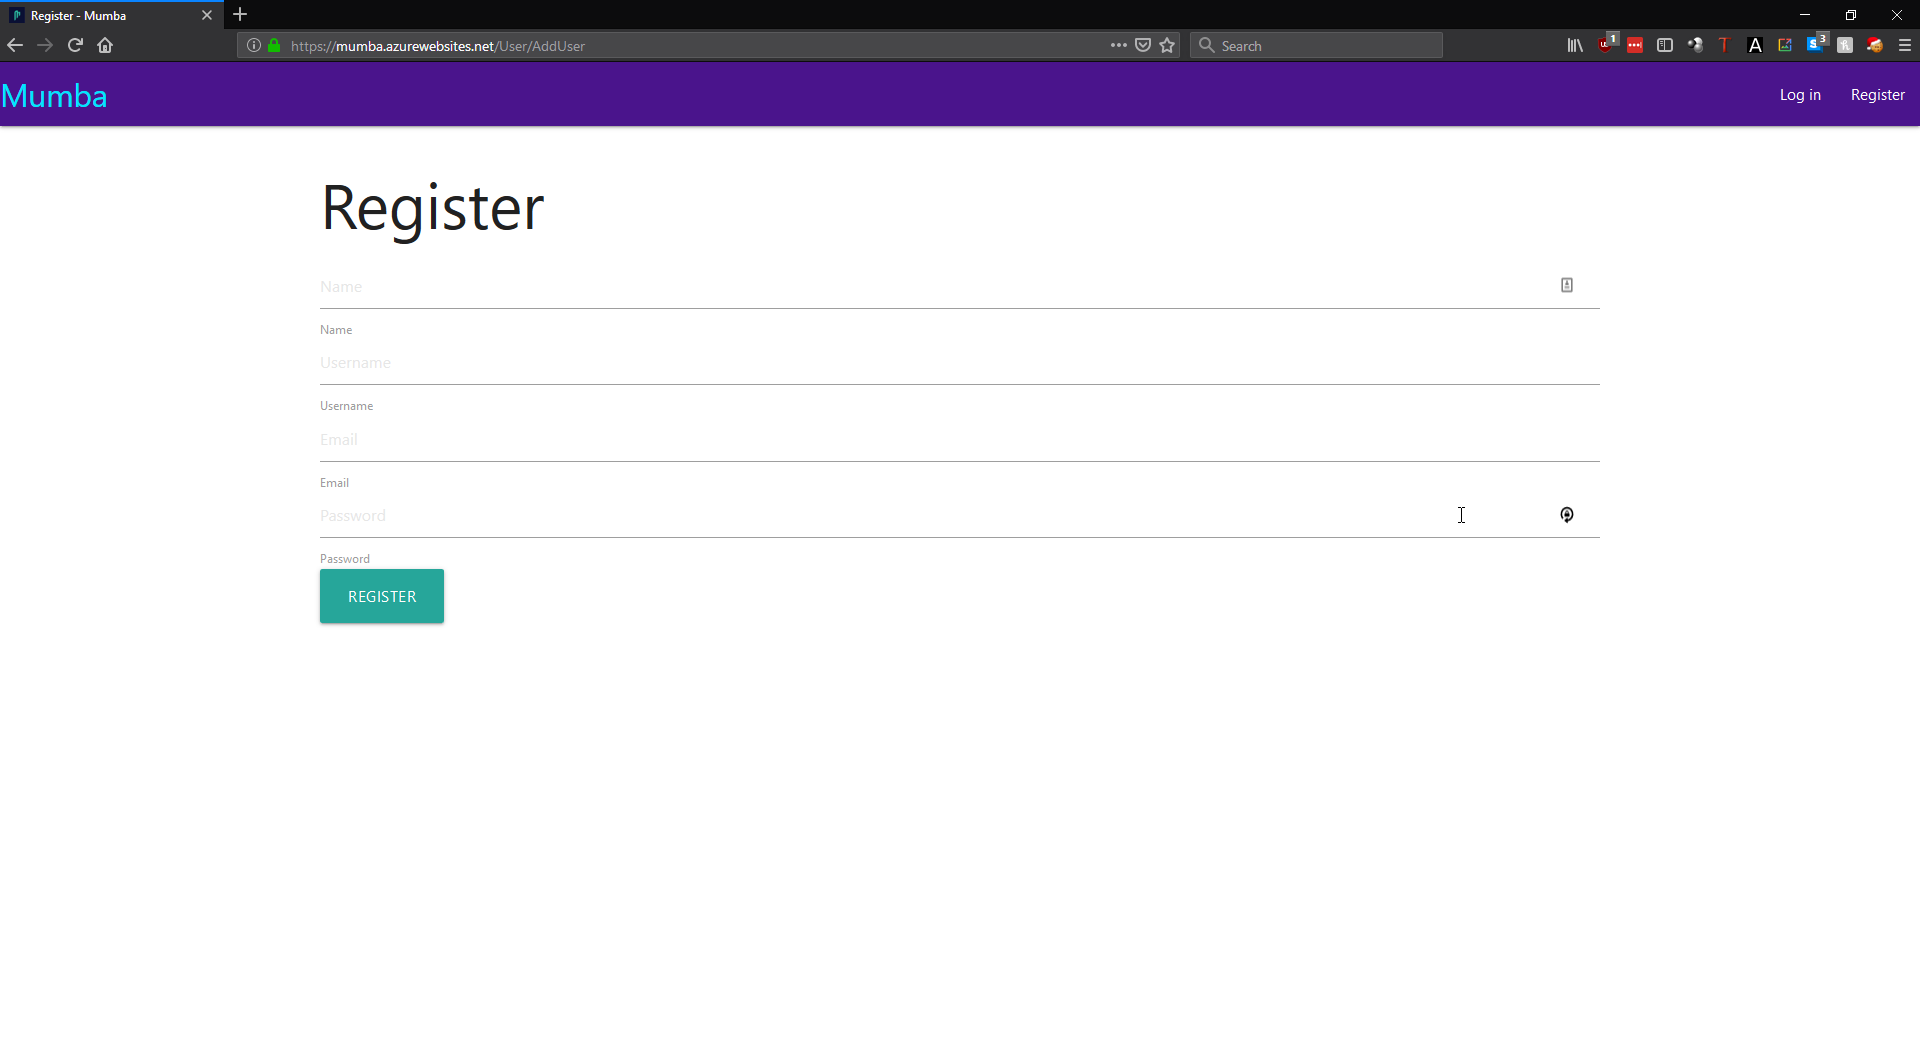
\includegraphics[scale=0.2]{Images/Register}
\end{figure}


\subsection{Boards}

\subsubsection{All}
\begin{figure}[H]
  \centering
  \caption{The All Boards View}
  \includegraphics[scale=0.2]{Images/"Your Boards"}
\end{figure}
\subsubsection{Open}
\begin{figure}[H]
  \centering
  \caption{The Open Board View}
  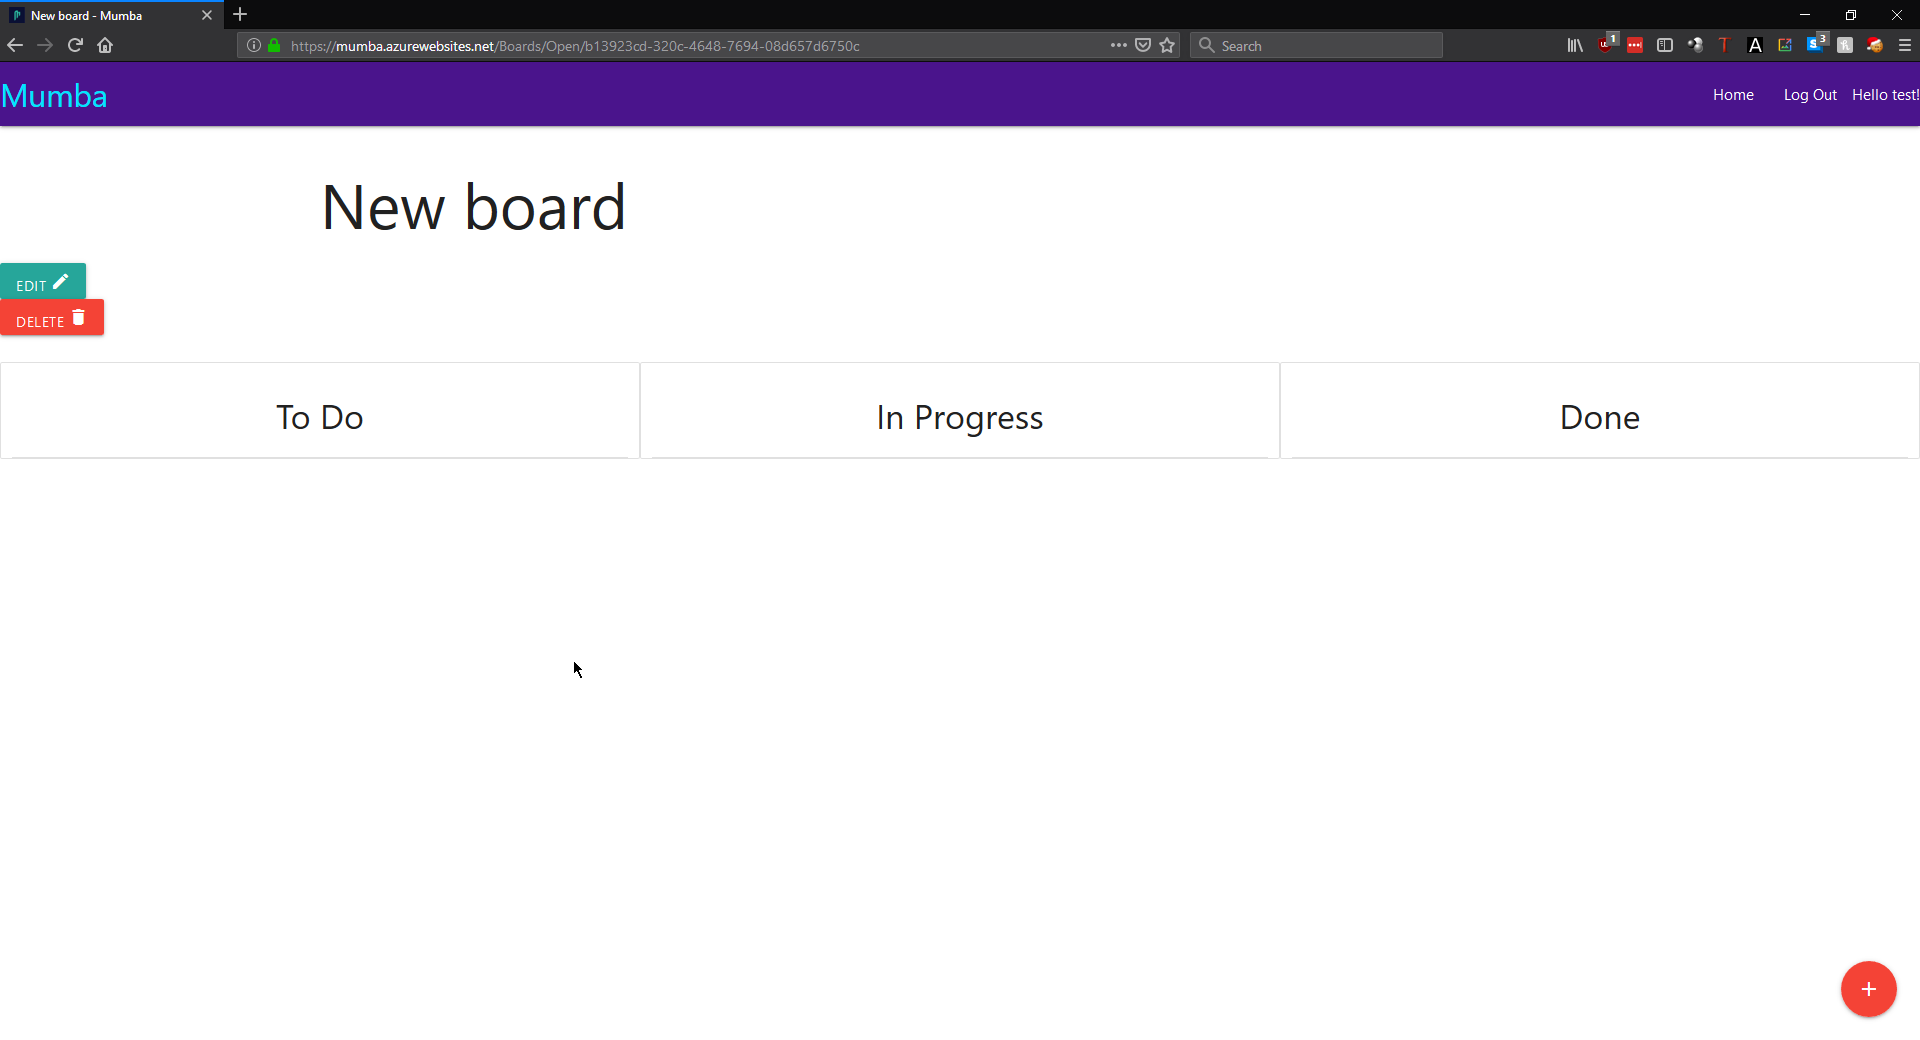
\includegraphics[scale=0.2]{Images/BlankBoard}
\end{figure}
\subsubsection{Add}
\begin{figure}[H]
  \centering
  \caption{The Board Creation View}
  \includegraphics[scale=0.2]{Images/"Add Board"}
\end{figure}
\subsubsection{Edit}
\begin{figure}[H]
  \centering
  \caption{The Board Edit View}
  \includegraphics[scale=0.2]{Images/"Edit Board"}
\end{figure}
\subsubsection{Delete}

\subsection{Tasks}

\subsubsection{Open}
\begin{figure}[H]
  \centering
  \caption{The Task Open View}
  \includegraphics[scale=0.2]{Images/"Task_ Task"}
\end{figure}
\subsubsection{Add}

\begin{figure}[H]
  \centering
  \caption{The Add Task View}
  \includegraphics[scale=0.2]{Images/"Add Task"}
\end{figure}
\subsubsection{Edit}

\begin{figure}[H]
  \centering
  \caption{The Task Edit View}
  \includegraphics[scale=0.2]{Images/"Edit Task"}
\end{figure}
\subsubsection{Delete}






\pagebreak
\section{Conclusion}
The final implementation of Mumba delivers a fully functional web application hosted at https://mumba.azurewebsites.net that meets the goals of providing a simple and easy to use project management solution. The service is very secure, with security as a choice from the very beginning. Using the Microsoft Identity package the website handles session management and data security natively. I used the CSS grid to create the many different elements of my pages, and in doing so made my website responsive, it will function and look good on any screen size. The main areas that Mumba could be improved are the following:
\begin{itemize}
  \item One: Allow the dynamic creation/deletion/naming of lists within boards.
  \item Two: Create a method of sharing boards between two or more users to allow collaborative projects to be managed in Mumba
\end{itemize}
Once both of these features are implemented Mumba would be in a state that I would consider feature complete, anything else that would be added would just be extra.

\end{document}
